% Options for packages loaded elsewhere
\PassOptionsToPackage{unicode}{hyperref}
\PassOptionsToPackage{hyphens}{url}
\PassOptionsToPackage{dvipsnames,svgnames,x11names}{xcolor}
%
\documentclass[
  letterpaper,
  DIV=11,
  numbers=noendperiod]{scrreprt}

\usepackage{amsmath,amssymb}
\usepackage{iftex}
\ifPDFTeX
  \usepackage[T1]{fontenc}
  \usepackage[utf8]{inputenc}
  \usepackage{textcomp} % provide euro and other symbols
\else % if luatex or xetex
  \usepackage{unicode-math}
  \defaultfontfeatures{Scale=MatchLowercase}
  \defaultfontfeatures[\rmfamily]{Ligatures=TeX,Scale=1}
\fi
\usepackage{lmodern}
\ifPDFTeX\else  
    % xetex/luatex font selection
\fi
% Use upquote if available, for straight quotes in verbatim environments
\IfFileExists{upquote.sty}{\usepackage{upquote}}{}
\IfFileExists{microtype.sty}{% use microtype if available
  \usepackage[]{microtype}
  \UseMicrotypeSet[protrusion]{basicmath} % disable protrusion for tt fonts
}{}
\makeatletter
\@ifundefined{KOMAClassName}{% if non-KOMA class
  \IfFileExists{parskip.sty}{%
    \usepackage{parskip}
  }{% else
    \setlength{\parindent}{0pt}
    \setlength{\parskip}{6pt plus 2pt minus 1pt}}
}{% if KOMA class
  \KOMAoptions{parskip=half}}
\makeatother
\usepackage{xcolor}
\setlength{\emergencystretch}{3em} % prevent overfull lines
\setcounter{secnumdepth}{5}
% Make \paragraph and \subparagraph free-standing
\makeatletter
\ifx\paragraph\undefined\else
  \let\oldparagraph\paragraph
  \renewcommand{\paragraph}{
    \@ifstar
      \xxxParagraphStar
      \xxxParagraphNoStar
  }
  \newcommand{\xxxParagraphStar}[1]{\oldparagraph*{#1}\mbox{}}
  \newcommand{\xxxParagraphNoStar}[1]{\oldparagraph{#1}\mbox{}}
\fi
\ifx\subparagraph\undefined\else
  \let\oldsubparagraph\subparagraph
  \renewcommand{\subparagraph}{
    \@ifstar
      \xxxSubParagraphStar
      \xxxSubParagraphNoStar
  }
  \newcommand{\xxxSubParagraphStar}[1]{\oldsubparagraph*{#1}\mbox{}}
  \newcommand{\xxxSubParagraphNoStar}[1]{\oldsubparagraph{#1}\mbox{}}
\fi
\makeatother

\usepackage{color}
\usepackage{fancyvrb}
\newcommand{\VerbBar}{|}
\newcommand{\VERB}{\Verb[commandchars=\\\{\}]}
\DefineVerbatimEnvironment{Highlighting}{Verbatim}{commandchars=\\\{\}}
% Add ',fontsize=\small' for more characters per line
\usepackage{framed}
\definecolor{shadecolor}{RGB}{241,243,245}
\newenvironment{Shaded}{\begin{snugshade}}{\end{snugshade}}
\newcommand{\AlertTok}[1]{\textcolor[rgb]{0.68,0.00,0.00}{#1}}
\newcommand{\AnnotationTok}[1]{\textcolor[rgb]{0.37,0.37,0.37}{#1}}
\newcommand{\AttributeTok}[1]{\textcolor[rgb]{0.40,0.45,0.13}{#1}}
\newcommand{\BaseNTok}[1]{\textcolor[rgb]{0.68,0.00,0.00}{#1}}
\newcommand{\BuiltInTok}[1]{\textcolor[rgb]{0.00,0.23,0.31}{#1}}
\newcommand{\CharTok}[1]{\textcolor[rgb]{0.13,0.47,0.30}{#1}}
\newcommand{\CommentTok}[1]{\textcolor[rgb]{0.37,0.37,0.37}{#1}}
\newcommand{\CommentVarTok}[1]{\textcolor[rgb]{0.37,0.37,0.37}{\textit{#1}}}
\newcommand{\ConstantTok}[1]{\textcolor[rgb]{0.56,0.35,0.01}{#1}}
\newcommand{\ControlFlowTok}[1]{\textcolor[rgb]{0.00,0.23,0.31}{\textbf{#1}}}
\newcommand{\DataTypeTok}[1]{\textcolor[rgb]{0.68,0.00,0.00}{#1}}
\newcommand{\DecValTok}[1]{\textcolor[rgb]{0.68,0.00,0.00}{#1}}
\newcommand{\DocumentationTok}[1]{\textcolor[rgb]{0.37,0.37,0.37}{\textit{#1}}}
\newcommand{\ErrorTok}[1]{\textcolor[rgb]{0.68,0.00,0.00}{#1}}
\newcommand{\ExtensionTok}[1]{\textcolor[rgb]{0.00,0.23,0.31}{#1}}
\newcommand{\FloatTok}[1]{\textcolor[rgb]{0.68,0.00,0.00}{#1}}
\newcommand{\FunctionTok}[1]{\textcolor[rgb]{0.28,0.35,0.67}{#1}}
\newcommand{\ImportTok}[1]{\textcolor[rgb]{0.00,0.46,0.62}{#1}}
\newcommand{\InformationTok}[1]{\textcolor[rgb]{0.37,0.37,0.37}{#1}}
\newcommand{\KeywordTok}[1]{\textcolor[rgb]{0.00,0.23,0.31}{\textbf{#1}}}
\newcommand{\NormalTok}[1]{\textcolor[rgb]{0.00,0.23,0.31}{#1}}
\newcommand{\OperatorTok}[1]{\textcolor[rgb]{0.37,0.37,0.37}{#1}}
\newcommand{\OtherTok}[1]{\textcolor[rgb]{0.00,0.23,0.31}{#1}}
\newcommand{\PreprocessorTok}[1]{\textcolor[rgb]{0.68,0.00,0.00}{#1}}
\newcommand{\RegionMarkerTok}[1]{\textcolor[rgb]{0.00,0.23,0.31}{#1}}
\newcommand{\SpecialCharTok}[1]{\textcolor[rgb]{0.37,0.37,0.37}{#1}}
\newcommand{\SpecialStringTok}[1]{\textcolor[rgb]{0.13,0.47,0.30}{#1}}
\newcommand{\StringTok}[1]{\textcolor[rgb]{0.13,0.47,0.30}{#1}}
\newcommand{\VariableTok}[1]{\textcolor[rgb]{0.07,0.07,0.07}{#1}}
\newcommand{\VerbatimStringTok}[1]{\textcolor[rgb]{0.13,0.47,0.30}{#1}}
\newcommand{\WarningTok}[1]{\textcolor[rgb]{0.37,0.37,0.37}{\textit{#1}}}

\providecommand{\tightlist}{%
  \setlength{\itemsep}{0pt}\setlength{\parskip}{0pt}}\usepackage{longtable,booktabs,array}
\usepackage{calc} % for calculating minipage widths
% Correct order of tables after \paragraph or \subparagraph
\usepackage{etoolbox}
\makeatletter
\patchcmd\longtable{\par}{\if@noskipsec\mbox{}\fi\par}{}{}
\makeatother
% Allow footnotes in longtable head/foot
\IfFileExists{footnotehyper.sty}{\usepackage{footnotehyper}}{\usepackage{footnote}}
\makesavenoteenv{longtable}
\usepackage{graphicx}
\makeatletter
\def\maxwidth{\ifdim\Gin@nat@width>\linewidth\linewidth\else\Gin@nat@width\fi}
\def\maxheight{\ifdim\Gin@nat@height>\textheight\textheight\else\Gin@nat@height\fi}
\makeatother
% Scale images if necessary, so that they will not overflow the page
% margins by default, and it is still possible to overwrite the defaults
% using explicit options in \includegraphics[width, height, ...]{}
\setkeys{Gin}{width=\maxwidth,height=\maxheight,keepaspectratio}
% Set default figure placement to htbp
\makeatletter
\def\fps@figure{htbp}
\makeatother
% definitions for citeproc citations
\NewDocumentCommand\citeproctext{}{}
\NewDocumentCommand\citeproc{mm}{%
  \begingroup\def\citeproctext{#2}\cite{#1}\endgroup}
\makeatletter
 % allow citations to break across lines
 \let\@cite@ofmt\@firstofone
 % avoid brackets around text for \cite:
 \def\@biblabel#1{}
 \def\@cite#1#2{{#1\if@tempswa , #2\fi}}
\makeatother
\newlength{\cslhangindent}
\setlength{\cslhangindent}{1.5em}
\newlength{\csllabelwidth}
\setlength{\csllabelwidth}{3em}
\newenvironment{CSLReferences}[2] % #1 hanging-indent, #2 entry-spacing
 {\begin{list}{}{%
  \setlength{\itemindent}{0pt}
  \setlength{\leftmargin}{0pt}
  \setlength{\parsep}{0pt}
  % turn on hanging indent if param 1 is 1
  \ifodd #1
   \setlength{\leftmargin}{\cslhangindent}
   \setlength{\itemindent}{-1\cslhangindent}
  \fi
  % set entry spacing
  \setlength{\itemsep}{#2\baselineskip}}}
 {\end{list}}
\usepackage{calc}
\newcommand{\CSLBlock}[1]{\hfill\break\parbox[t]{\linewidth}{\strut\ignorespaces#1\strut}}
\newcommand{\CSLLeftMargin}[1]{\parbox[t]{\csllabelwidth}{\strut#1\strut}}
\newcommand{\CSLRightInline}[1]{\parbox[t]{\linewidth - \csllabelwidth}{\strut#1\strut}}
\newcommand{\CSLIndent}[1]{\hspace{\cslhangindent}#1}

\KOMAoption{captions}{tableheading}
\makeatletter
\@ifpackageloaded{bookmark}{}{\usepackage{bookmark}}
\makeatother
\makeatletter
\@ifpackageloaded{caption}{}{\usepackage{caption}}
\AtBeginDocument{%
\ifdefined\contentsname
  \renewcommand*\contentsname{Table of contents}
\else
  \newcommand\contentsname{Table of contents}
\fi
\ifdefined\listfigurename
  \renewcommand*\listfigurename{List of Figures}
\else
  \newcommand\listfigurename{List of Figures}
\fi
\ifdefined\listtablename
  \renewcommand*\listtablename{List of Tables}
\else
  \newcommand\listtablename{List of Tables}
\fi
\ifdefined\figurename
  \renewcommand*\figurename{Figure}
\else
  \newcommand\figurename{Figure}
\fi
\ifdefined\tablename
  \renewcommand*\tablename{Table}
\else
  \newcommand\tablename{Table}
\fi
}
\@ifpackageloaded{float}{}{\usepackage{float}}
\floatstyle{ruled}
\@ifundefined{c@chapter}{\newfloat{codelisting}{h}{lop}}{\newfloat{codelisting}{h}{lop}[chapter]}
\floatname{codelisting}{Listing}
\newcommand*\listoflistings{\listof{codelisting}{List of Listings}}
\makeatother
\makeatletter
\makeatother
\makeatletter
\@ifpackageloaded{caption}{}{\usepackage{caption}}
\@ifpackageloaded{subcaption}{}{\usepackage{subcaption}}
\makeatother

\ifLuaTeX
  \usepackage{selnolig}  % disable illegal ligatures
\fi
\usepackage{bookmark}

\IfFileExists{xurl.sty}{\usepackage{xurl}}{} % add URL line breaks if available
\urlstyle{same} % disable monospaced font for URLs
\hypersetup{
  pdftitle={dswg-book},
  pdfauthor={Norah Jones},
  colorlinks=true,
  linkcolor={blue},
  filecolor={Maroon},
  citecolor={Blue},
  urlcolor={Blue},
  pdfcreator={LaTeX via pandoc}}


\title{dswg-book}
\author{Norah Jones}
\date{2024-10-16}

\begin{document}
\maketitle

\renewcommand*\contentsname{Table of contents}
{
\hypersetup{linkcolor=}
\setcounter{tocdepth}{2}
\tableofcontents
}

\bookmarksetup{startatroot}

\chapter*{Preface}\label{preface}
\addcontentsline{toc}{chapter}{Preface}

\markboth{Preface}{Preface}

This is a Quarto book.

To learn more about Quarto books visit
\url{https://quarto.org/docs/books}.

\begin{Shaded}
\begin{Highlighting}[]
\DecValTok{1} \SpecialCharTok{+} \DecValTok{1}
\end{Highlighting}
\end{Shaded}

\begin{verbatim}
[1] 2
\end{verbatim}

\bookmarksetup{startatroot}

\chapter{Introduction}\label{introduction}

This is a book created from markdown and executable code.

See Knuth (1984) for additional discussion of literate programming.

\begin{Shaded}
\begin{Highlighting}[]
\DecValTok{1} \SpecialCharTok{+} \DecValTok{1}
\end{Highlighting}
\end{Shaded}

\begin{verbatim}
[1] 2
\end{verbatim}

\bookmarksetup{startatroot}

\chapter{Summary}\label{summary}

In summary, this book has no content whatsoever.

\begin{Shaded}
\begin{Highlighting}[]
\DecValTok{1} \SpecialCharTok{+} \DecValTok{1}
\end{Highlighting}
\end{Shaded}

\begin{verbatim}
[1] 2
\end{verbatim}

\bookmarksetup{startatroot}

\chapter*{References}\label{references}
\addcontentsline{toc}{chapter}{References}

\markboth{References}{References}

\phantomsection\label{refs}
\begin{CSLReferences}{1}{0}
\bibitem[\citeproctext]{ref-knuth84}
Knuth, Donald E. 1984. {``Literate Programming.''} \emph{Comput. J.} 27
(2): 97--111. \url{https://doi.org/10.1093/comjnl/27.2.97}.

\end{CSLReferences}

\bookmarksetup{startatroot}

\chapter{actuar}\label{actuar}

\section{パッケージの概要}\label{ux30d1ux30c3ux30b1ux30fcux30b8ux306eux6982ux8981}

actuar パッケージは、stats
パッケージに収録されていない確率分布を扱うための関数を実装したパッケージです。特に、パレート分布、Burr分布、対数ガンマ分布、対数ロジスティック分布など、裾の厚い分布が数多く収録されています。

なお、\texttt{d****(x,\ ...)} が密度関数、\texttt{p****(x,\ ...)}
が累積分布関数、\texttt{r****(n,\ ...)} が乱数、\texttt{q(p,\ ...)}
が分位点を表しているのは stats パッケージと同じです。

\section{確率密度関数をプロットする}\label{ux78baux7387ux5bc6ux5ea6ux95a2ux6570ux3092ux30d7ux30edux30c3ux30c8ux3059ux308b}

\begin{itemize}
\tightlist
\item
  パレート分布 \texttt{pareto}\\
  \[dpareto(x,{\alpha},{\theta})={{\alpha}{\theta}^{\alpha}}/{(x+\theta)^{\alpha+1}}\]
\end{itemize}

\begin{Shaded}
\begin{Highlighting}[]
\FunctionTok{library}\NormalTok{(actuar)}

\NormalTok{xlim }\OtherTok{\textless{}{-}} \FunctionTok{c}\NormalTok{(}\DecValTok{0}\NormalTok{, }\DecValTok{3}\NormalTok{)}
\NormalTok{ylim }\OtherTok{\textless{}{-}} \FunctionTok{c}\NormalTok{(}\DecValTok{0}\NormalTok{, }\DecValTok{2}\NormalTok{)}
\NormalTok{main }\OtherTok{\textless{}{-}} \StringTok{"pareto distribution"}

\FunctionTok{curve}\NormalTok{(}\FunctionTok{dpareto}\NormalTok{(x, }\DecValTok{1}\NormalTok{, }\DecValTok{1}\NormalTok{), }\AttributeTok{type =} \StringTok{"l"}\NormalTok{, }\AttributeTok{lty =} \DecValTok{1}\NormalTok{, }\AttributeTok{col =} \StringTok{"darkgray"}\NormalTok{,}
      \AttributeTok{xlim =}\NormalTok{ xlim, }\AttributeTok{ylim =}\NormalTok{ ylim, }\AttributeTok{ylab =} \StringTok{""}\NormalTok{, }\AttributeTok{main =}\NormalTok{ main)}
\FunctionTok{curve}\NormalTok{(}\FunctionTok{dpareto}\NormalTok{(x, }\DecValTok{2}\NormalTok{, }\DecValTok{1}\NormalTok{), }\AttributeTok{type =} \StringTok{"l"}\NormalTok{, }\AttributeTok{lty =} \DecValTok{2}\NormalTok{, }\AttributeTok{col =} \StringTok{"darkcyan"}\NormalTok{, }\AttributeTok{add =} \ConstantTok{TRUE}\NormalTok{)}
\FunctionTok{curve}\NormalTok{(}\FunctionTok{dpareto}\NormalTok{(x, }\DecValTok{1}\NormalTok{, }\DecValTok{2}\NormalTok{), }\AttributeTok{type =} \StringTok{"l"}\NormalTok{, }\AttributeTok{lty =} \DecValTok{3}\NormalTok{, }\AttributeTok{col =} \StringTok{"darkred"}\NormalTok{, }\AttributeTok{add =} \ConstantTok{TRUE}\NormalTok{)}
\FunctionTok{curve}\NormalTok{(}\FunctionTok{dpareto}\NormalTok{(x, }\DecValTok{2}\NormalTok{, }\DecValTok{2}\NormalTok{), }\AttributeTok{type =} \StringTok{"l"}\NormalTok{, }\AttributeTok{lty =} \DecValTok{4}\NormalTok{, }\AttributeTok{col =} \StringTok{"darkblue"}\NormalTok{, }\AttributeTok{add =} \ConstantTok{TRUE}\NormalTok{)}
\end{Highlighting}
\end{Shaded}

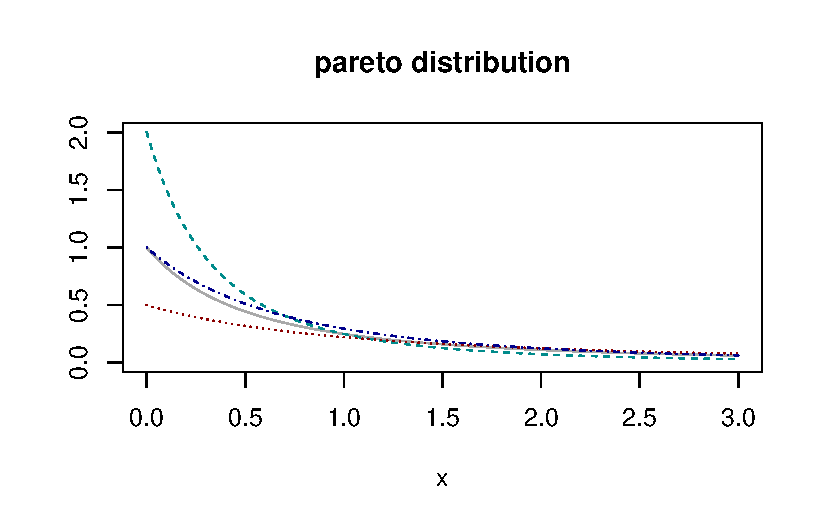
\includegraphics{actuar_files/figure-pdf/pareto-1.pdf}

\begin{itemize}
\tightlist
\item
  Burr分布 \texttt{burr}\\
  \[dburr(x,{\alpha},{\gamma},{\theta})={{\alpha}{\gamma}(x/{\theta})^{\gamma}}/{x[1+(x/{\theta)^{\gamma}}]^{\alpha + 1}}\]
\end{itemize}

\begin{Shaded}
\begin{Highlighting}[]
\NormalTok{xlim }\OtherTok{\textless{}{-}} \FunctionTok{c}\NormalTok{(}\DecValTok{0}\NormalTok{, }\DecValTok{3}\NormalTok{)}
\NormalTok{ylim }\OtherTok{\textless{}{-}} \FunctionTok{c}\NormalTok{(}\DecValTok{0}\NormalTok{, }\DecValTok{2}\NormalTok{)}
\NormalTok{main }\OtherTok{\textless{}{-}} \StringTok{"burr distribution"}

\FunctionTok{curve}\NormalTok{(}\FunctionTok{dburr}\NormalTok{(x, }\DecValTok{1}\NormalTok{, }\DecValTok{1}\NormalTok{, }\DecValTok{1}\NormalTok{), }\AttributeTok{type =} \StringTok{"l"}\NormalTok{, }\AttributeTok{lty =} \DecValTok{1}\NormalTok{, }\AttributeTok{col =} \StringTok{"darkgray"}\NormalTok{,}
      \AttributeTok{xlim =}\NormalTok{ xlim, }\AttributeTok{ylim =}\NormalTok{ ylim, }\AttributeTok{ylab =} \StringTok{""}\NormalTok{, }\AttributeTok{main =}\NormalTok{ main)}
\FunctionTok{curve}\NormalTok{(}\FunctionTok{dburr}\NormalTok{(x, }\DecValTok{2}\NormalTok{, }\DecValTok{1}\NormalTok{, }\DecValTok{1}\NormalTok{), }\AttributeTok{type =} \StringTok{"l"}\NormalTok{, }\AttributeTok{lty =} \DecValTok{2}\NormalTok{, }\AttributeTok{col =} \StringTok{"darkcyan"}\NormalTok{, }\AttributeTok{add =} \ConstantTok{TRUE}\NormalTok{)}
\FunctionTok{curve}\NormalTok{(}\FunctionTok{dburr}\NormalTok{(x, }\DecValTok{1}\NormalTok{, }\DecValTok{2}\NormalTok{, }\DecValTok{2}\NormalTok{), }\AttributeTok{type =} \StringTok{"l"}\NormalTok{, }\AttributeTok{lty =} \DecValTok{3}\NormalTok{, }\AttributeTok{col =} \StringTok{"darkred"}\NormalTok{, }\AttributeTok{add =} \ConstantTok{TRUE}\NormalTok{)}
\FunctionTok{curve}\NormalTok{(}\FunctionTok{dburr}\NormalTok{(x, }\DecValTok{2}\NormalTok{, }\DecValTok{2}\NormalTok{, }\DecValTok{2}\NormalTok{), }\AttributeTok{type =} \StringTok{"l"}\NormalTok{, }\AttributeTok{lty =} \DecValTok{4}\NormalTok{, }\AttributeTok{col =} \StringTok{"darkblue"}\NormalTok{, }\AttributeTok{add =} \ConstantTok{TRUE}\NormalTok{)}
\end{Highlighting}
\end{Shaded}

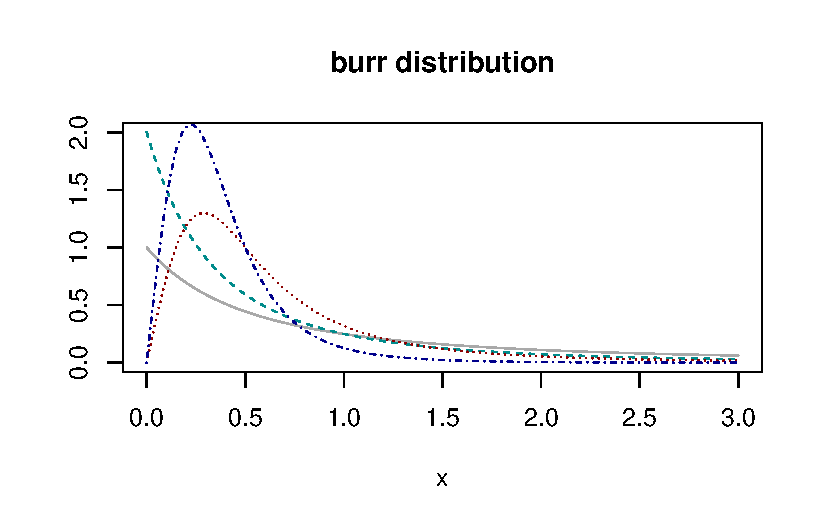
\includegraphics{actuar_files/figure-pdf/burr-1.pdf}

\begin{itemize}
\tightlist
\item
  対数ガンマ分布 \texttt{lgamma}\\
  \[dlgamma(x,{\alpha},{\lambda})={{\lambda}^{\alpha}{\Gamma}({\alpha})}/{[(\log{x})^{\alpha-1}x^{\lambda+1}]}\]
\end{itemize}

\begin{Shaded}
\begin{Highlighting}[]
\NormalTok{xlim }\OtherTok{\textless{}{-}} \FunctionTok{c}\NormalTok{(}\DecValTok{1}\NormalTok{, }\DecValTok{4}\NormalTok{)}
\NormalTok{ylim }\OtherTok{\textless{}{-}} \FunctionTok{c}\NormalTok{(}\DecValTok{0}\NormalTok{, }\DecValTok{2}\NormalTok{)}
\NormalTok{main }\OtherTok{\textless{}{-}} \StringTok{"log gamma distribution"}

\FunctionTok{curve}\NormalTok{(}\FunctionTok{dlgamma}\NormalTok{(x, }\DecValTok{1}\NormalTok{, }\DecValTok{1}\NormalTok{), }\AttributeTok{type =} \StringTok{"l"}\NormalTok{, }\AttributeTok{lty =} \DecValTok{1}\NormalTok{, }\AttributeTok{col =} \StringTok{"darkgray"}\NormalTok{,}
      \AttributeTok{xlim =}\NormalTok{ xlim, }\AttributeTok{ylim =}\NormalTok{ ylim, }\AttributeTok{ylab =} \StringTok{""}\NormalTok{, }\AttributeTok{main =}\NormalTok{ main)}
\FunctionTok{curve}\NormalTok{(}\FunctionTok{dlgamma}\NormalTok{(x, }\DecValTok{2}\NormalTok{, }\DecValTok{1}\NormalTok{), }\AttributeTok{type =} \StringTok{"l"}\NormalTok{, }\AttributeTok{lty =} \DecValTok{2}\NormalTok{, }\AttributeTok{col =} \StringTok{"darkcyan"}\NormalTok{, }\AttributeTok{add =} \ConstantTok{TRUE}\NormalTok{)}
\FunctionTok{curve}\NormalTok{(}\FunctionTok{dlgamma}\NormalTok{(x, }\DecValTok{1}\NormalTok{, }\DecValTok{2}\NormalTok{), }\AttributeTok{type =} \StringTok{"l"}\NormalTok{, }\AttributeTok{lty =} \DecValTok{3}\NormalTok{, }\AttributeTok{col =} \StringTok{"darkred"}\NormalTok{, }\AttributeTok{add =} \ConstantTok{TRUE}\NormalTok{)}
\FunctionTok{curve}\NormalTok{(}\FunctionTok{dlgamma}\NormalTok{(x, }\DecValTok{2}\NormalTok{, }\DecValTok{2}\NormalTok{), }\AttributeTok{type =} \StringTok{"l"}\NormalTok{, }\AttributeTok{lty =} \DecValTok{4}\NormalTok{, }\AttributeTok{col =} \StringTok{"darkblue"}\NormalTok{, }\AttributeTok{add =} \ConstantTok{TRUE}\NormalTok{)}
\end{Highlighting}
\end{Shaded}

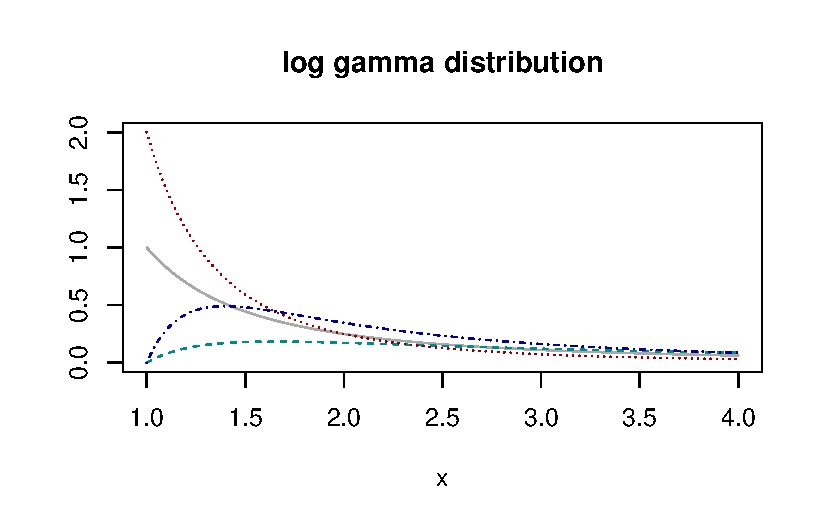
\includegraphics{actuar_files/figure-pdf/loggamma-1.pdf}

\begin{itemize}
\tightlist
\item
  対数ロジスティック分布 \texttt{llogis}\\
  \[dllogis(x,{\gamma},{\theta})={{\gamma}(x/{\theta})^{\gamma}}/{x[1+(x/{\theta)}]^2}\]
\end{itemize}

\begin{Shaded}
\begin{Highlighting}[]
\NormalTok{xlim }\OtherTok{\textless{}{-}} \FunctionTok{c}\NormalTok{(}\DecValTok{0}\NormalTok{, }\DecValTok{3}\NormalTok{)}
\NormalTok{ylim }\OtherTok{\textless{}{-}} \FunctionTok{c}\NormalTok{(}\DecValTok{0}\NormalTok{, }\DecValTok{2}\NormalTok{)}
\NormalTok{main }\OtherTok{\textless{}{-}} \StringTok{"log logistic distribution"}

\FunctionTok{curve}\NormalTok{(}\FunctionTok{dllogis}\NormalTok{(x, }\DecValTok{1}\NormalTok{, }\DecValTok{1}\NormalTok{), }\AttributeTok{type =} \StringTok{"l"}\NormalTok{, }\AttributeTok{lty =} \DecValTok{1}\NormalTok{, }\AttributeTok{col =} \StringTok{"darkgray"}\NormalTok{,}
      \AttributeTok{xlim =}\NormalTok{ xlim, }\AttributeTok{ylim =}\NormalTok{ ylim, }\AttributeTok{ylab =} \StringTok{""}\NormalTok{, }\AttributeTok{main =}\NormalTok{ main)}
\FunctionTok{curve}\NormalTok{(}\FunctionTok{dllogis}\NormalTok{(x, }\DecValTok{2}\NormalTok{, }\DecValTok{1}\NormalTok{), }\AttributeTok{type =} \StringTok{"l"}\NormalTok{, }\AttributeTok{lty =} \DecValTok{2}\NormalTok{, }\AttributeTok{col =} \StringTok{"darkcyan"}\NormalTok{, }\AttributeTok{add =} \ConstantTok{TRUE}\NormalTok{)}
\FunctionTok{curve}\NormalTok{(}\FunctionTok{dllogis}\NormalTok{(x, }\DecValTok{1}\NormalTok{, }\DecValTok{2}\NormalTok{), }\AttributeTok{type =} \StringTok{"l"}\NormalTok{, }\AttributeTok{lty =} \DecValTok{3}\NormalTok{, }\AttributeTok{col =} \StringTok{"darkred"}\NormalTok{, }\AttributeTok{add =} \ConstantTok{TRUE}\NormalTok{)}
\FunctionTok{curve}\NormalTok{(}\FunctionTok{dllogis}\NormalTok{(x, }\DecValTok{2}\NormalTok{, }\DecValTok{2}\NormalTok{), }\AttributeTok{type =} \StringTok{"l"}\NormalTok{, }\AttributeTok{lty =} \DecValTok{4}\NormalTok{, }\AttributeTok{col =} \StringTok{"darkblue"}\NormalTok{, }\AttributeTok{add =} \ConstantTok{TRUE}\NormalTok{)}
\end{Highlighting}
\end{Shaded}

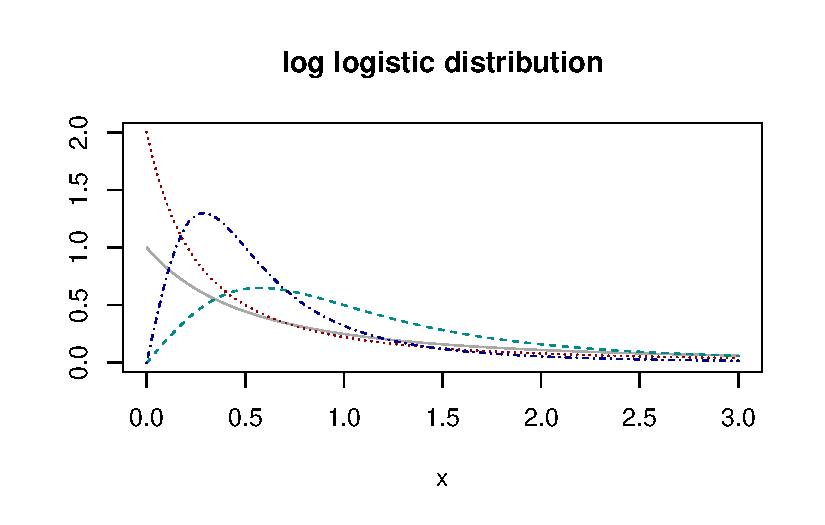
\includegraphics{actuar_files/figure-pdf/logistic-1.pdf}

actuar
パッケージには、これらのほかにも以下のような確率分布が実装されています。

\begin{itemize}
\item
  逆ガンマ分布 \texttt{invgamma}
\item
  逆パレート分布 \texttt{invpareto}
\item
  逆バー分布 \texttt{invburr}
\item
  逆ワイブル分布 \texttt{invweibull}
\item
  逆指数分布 \texttt{invexp}
\item
  一般化ベータ分布 \texttt{genbeta}
\item
  一般化パレート分布 \texttt{genpareto}\\
\end{itemize}

\bookmarksetup{startatroot}

\chapter{aglm}\label{aglm}

\section{パッケージの概要}\label{ux30d1ux30c3ux30b1ux30fcux30b8ux306eux6982ux8981-1}

aglm パッケージは、Accurate Generalized Linear Model (AGLM)
を実装したパッケージです。AGLM
は、加法的モデルの枠組にとどまることで一定の解釈性を維持しながら、目的変数と予測変数の間の非線形な関係を表現することで予測精度の向上もねらうことのできる予測モデルです。

\begin{Shaded}
\begin{Highlighting}[]
\FunctionTok{library}\NormalTok{(ggplot2)}
\FunctionTok{library}\NormalTok{(MASS) }\CommentTok{\# Bostonデータセットを利用します}

\FunctionTok{set.seed}\NormalTok{(}\DecValTok{42}\NormalTok{)}
\CommentTok{\# 学習用データと評価用データを分割します。}
\NormalTok{split\_data }\OtherTok{\textless{}{-}}\NormalTok{ rsample}\SpecialCharTok{::}\FunctionTok{initial\_split}\NormalTok{(Boston)}

\CommentTok{\# 学習用データを説明変数（デザイン行列）と目的変数に分割します。}
\NormalTok{train }\OtherTok{\textless{}{-}}\NormalTok{ rsample}\SpecialCharTok{::}\FunctionTok{training}\NormalTok{(split\_data)}
\NormalTok{train\_X }\OtherTok{\textless{}{-}}\NormalTok{ dplyr}\SpecialCharTok{::}\FunctionTok{select}\NormalTok{(train, }\SpecialCharTok{{-}}\NormalTok{medv)}
\NormalTok{train\_y }\OtherTok{\textless{}{-}}\NormalTok{ train}\SpecialCharTok{$}\NormalTok{medv}

\CommentTok{\# 評価データを説明変数と目的変数に分割します。}
\NormalTok{test }\OtherTok{\textless{}{-}}\NormalTok{ rsample}\SpecialCharTok{::}\FunctionTok{testing}\NormalTok{(split\_data)}
\NormalTok{test\_X }\OtherTok{\textless{}{-}}\NormalTok{ dplyr}\SpecialCharTok{::}\FunctionTok{select}\NormalTok{(test, }\SpecialCharTok{{-}}\NormalTok{medv)}
\NormalTok{test\_y }\OtherTok{\textless{}{-}}\NormalTok{ test}\SpecialCharTok{$}\NormalTok{medv}
\end{Highlighting}
\end{Shaded}

\section{AGLM
モデルを構築する}\label{aglm-ux30e2ux30c7ux30ebux3092ux69cbux7bc9ux3059ux308b}

aglm関数の第1引数 \texttt{x} に説明変数（デザイン行列）を渡し、第2引数
\texttt{y}
に目的変数を渡すことで、AGLMを学習させることができます。また、\texttt{predict}
関数の引数 \texttt{newx}
に新たなデータを渡せば、そのデータに対する予測が出力されます。

\begin{Shaded}
\begin{Highlighting}[]
\FunctionTok{library}\NormalTok{(aglm)}

\NormalTok{model\_aglm }\OtherTok{\textless{}{-}} \FunctionTok{aglm}\NormalTok{(}
  \AttributeTok{x =}\NormalTok{ train\_X,}
  \AttributeTok{y =}\NormalTok{ train\_y,}
  \AttributeTok{alpha =} \DecValTok{1} \CommentTok{\# 正則化項のαパラメーターを指定（デフォルトは1）}
\NormalTok{  )}

\NormalTok{preds\_aglm }\OtherTok{\textless{}{-}} \FunctionTok{predict}\NormalTok{(}
  \AttributeTok{object =}\NormalTok{ model\_aglm,}
  \AttributeTok{newx =}\NormalTok{ test\_X,}
  \AttributeTok{s =} \FloatTok{0.1} \CommentTok{\# 正則化項のλパラメーターを数値またはベクトルで指定}
\NormalTok{) }\SpecialCharTok{|\textgreater{}} \FunctionTok{c}\NormalTok{() }\CommentTok{\# 行列形式の出力をベクトルに変換}

\NormalTok{rmse\_ }\OtherTok{=}\NormalTok{ yardstick}\SpecialCharTok{::}\FunctionTok{rmse\_vec}\NormalTok{(test\_y, preds\_aglm)}
\FunctionTok{ggplot}\NormalTok{(}\AttributeTok{mapping =} \FunctionTok{aes}\NormalTok{(}\AttributeTok{x =}\NormalTok{ test\_y, }\AttributeTok{y =}\NormalTok{ preds\_aglm)) }\SpecialCharTok{+}
  \FunctionTok{geom\_point}\NormalTok{() }\SpecialCharTok{+}
  \FunctionTok{labs}\NormalTok{(}\AttributeTok{title =} \FunctionTok{paste}\NormalTok{(}\StringTok{"AGLM Model: RMSE ="}\NormalTok{, }\FunctionTok{round}\NormalTok{(rmse\_, }\DecValTok{6}\NormalTok{)))}
\end{Highlighting}
\end{Shaded}

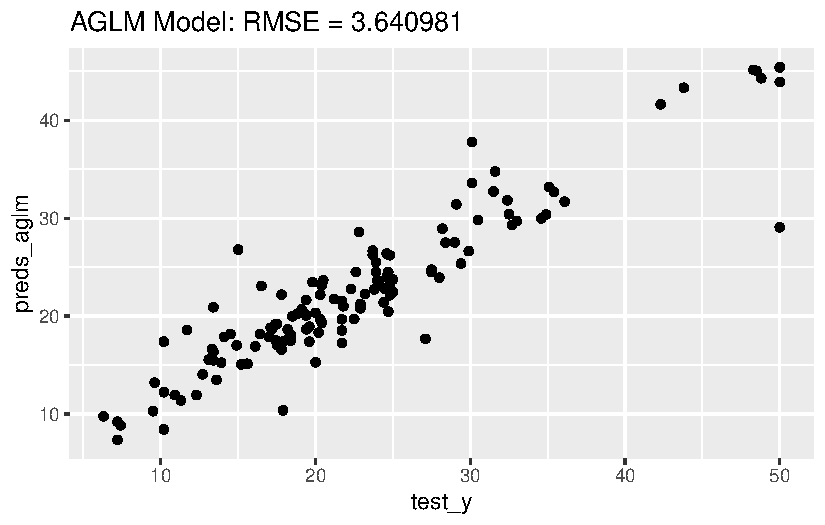
\includegraphics{aglm_files/figure-pdf/aglm-1.pdf}

\subsection{参考情報}\label{ux53c2ux8003ux60c5ux5831}

AGLMの学習における正則化項は次の式で与えられます。

\[R(\{\beta_{jk}\};\lambda, \alpha)=\lambda\{(1-\alpha)\sum_j\sum_k|\beta_{jk}|^2+\alpha\sum_j\sum_k|\beta_{jk}|\}\]

\(\alpha\)
はL1正則化とL2正則化のバランスを決めるパラメーターです。この形式の正則化項について、\(\alpha=1\)
の場合をラッソ、\(\alpha=0\) の場合をリッジ、\(0<\alpha<1\)
の場合をエラスティックネットと呼びます。また、λ
は正則化項の影響度を決めるパラメーターで、この値が大きいほど、回帰係数の値が小さく抑えられるようになります。

さて、AGLMでは、正則化項の λ
パラメーターを指定しない場合、デフォルトの設定では100通りの λ
の値に対して計算が行われます。

\begin{Shaded}
\begin{Highlighting}[]
\NormalTok{lambdas }\OtherTok{=}\NormalTok{ model\_aglm}\SpecialCharTok{@}\NormalTok{backend\_models}\SpecialCharTok{$}\NormalTok{glmnet}\SpecialCharTok{$}\NormalTok{lambda}
\FunctionTok{length}\NormalTok{(lambdas)}
\end{Highlighting}
\end{Shaded}

\begin{verbatim}
[1] 100
\end{verbatim}

\begin{Shaded}
\begin{Highlighting}[]
\NormalTok{lambdas[}\DecValTok{1}\SpecialCharTok{:}\DecValTok{5}\NormalTok{]}
\end{Highlighting}
\end{Shaded}

\begin{verbatim}
[1] 6.636452 6.334815 6.046888 5.772047 5.509699
\end{verbatim}

\begin{Shaded}
\begin{Highlighting}[]
\NormalTok{lambdas[}\DecValTok{96}\SpecialCharTok{:}\DecValTok{100}\NormalTok{]}
\end{Highlighting}
\end{Shaded}

\begin{verbatim}
[1] 0.07993630 0.07630307 0.07283498 0.06952452 0.06636452
\end{verbatim}

AGLMに predict() 関数を適用した場合の出力は、引数 s に渡した λ
パラメーターごとの予測値を 1 列として、行列形式で出力されます λ
の値を指定しない場合は、すべての λ
に対して予測が行われ、その結果が100列の行列として返されます。

\begin{Shaded}
\begin{Highlighting}[]
\FunctionTok{predict}\NormalTok{(model\_aglm, }\AttributeTok{newx =}\NormalTok{ test\_X) }\SpecialCharTok{|\textgreater{}} \FunctionTok{ncol}\NormalTok{()}
\end{Highlighting}
\end{Shaded}

\begin{verbatim}
[1] 100
\end{verbatim}

また、λ
パラメーターの値ごとに、学習の結果ゼロ以外の値になった回帰係数の数も記録されています。AGLM
では、非線形性を表現するために取り入れた工夫の影響で、推定される回帰係数の数（最大116）が、学習データに含まれる説明変数の数（13）よりも多くなります。

\begin{Shaded}
\begin{Highlighting}[]
\NormalTok{dfs }\OtherTok{=}\NormalTok{ model\_aglm}\SpecialCharTok{@}\NormalTok{backend\_models}\SpecialCharTok{$}\NormalTok{glmnet}\SpecialCharTok{$}\NormalTok{df}
\FunctionTok{length}\NormalTok{(dfs)}
\end{Highlighting}
\end{Shaded}

\begin{verbatim}
[1] 100
\end{verbatim}

\begin{Shaded}
\begin{Highlighting}[]
\NormalTok{dfs[}\DecValTok{1}\SpecialCharTok{:}\DecValTok{5}\NormalTok{]}
\end{Highlighting}
\end{Shaded}

\begin{verbatim}
[1] 0 1 1 2 2
\end{verbatim}

\begin{Shaded}
\begin{Highlighting}[]
\NormalTok{dfs[}\DecValTok{96}\SpecialCharTok{:}\DecValTok{100}\NormalTok{]}
\end{Highlighting}
\end{Shaded}

\begin{verbatim}
[1] 114 114 115 116 116
\end{verbatim}

なお、AGLM
では、非線形性を表現するために取り入れた工夫の影響で、推定される回帰係数の数（最大116）が、学習データに含まれる説明変数の数（13）よりも多くなります。この工夫の詳細については、AGLM
の紹介論文をご参照ください。

また、\(\alpha\) パラメーターが0でない場合、\(\lambda\)
が一定値を超えるとすべての回帰係数がゼロになります。このとき、AGLM
の予測関数は、説明変数の値によらずに目的変数の平均値を出力します。

\begin{Shaded}
\begin{Highlighting}[]
\FunctionTok{mean}\NormalTok{(train\_y)}
\end{Highlighting}
\end{Shaded}

\begin{verbatim}
[1] 22.44828
\end{verbatim}

\begin{Shaded}
\begin{Highlighting}[]
\FunctionTok{predict}\NormalTok{(model\_aglm, }\AttributeTok{newx =}\NormalTok{ test\_X,}
        \AttributeTok{s =} \FunctionTok{c}\NormalTok{(}\DecValTok{10}\NormalTok{, lambdas[}\DecValTok{1}\NormalTok{], lambdas[}\DecValTok{10}\NormalTok{])) }\SpecialCharTok{|\textgreater{}} \FunctionTok{head}\NormalTok{(}\DecValTok{3}\NormalTok{)}
\end{Highlighting}
\end{Shaded}

\begin{verbatim}
           s1       s2       s3
[1,] 22.44828 22.44828 21.98585
[2,] 22.44828 22.44828 20.34891
[3,] 22.44828 22.44828 21.18687
\end{verbatim}

\begin{Shaded}
\begin{Highlighting}[]
\CommentTok{\# 第1列（s1）はlambdas[1]以上の値を指定}
\end{Highlighting}
\end{Shaded}

\section{特徴量ごとの効果を可視化する}\label{ux7279ux5fb4ux91cfux3054ux3068ux306eux52b9ux679cux3092ux53efux8996ux5316ux3059ux308b}

構築した AGLM モデルを plot()
関数に渡すことで、特徴量ごとの予測値への影響を可視化することができます。

\begin{Shaded}
\begin{Highlighting}[]
\FunctionTok{plot}\NormalTok{(model\_aglm,}
     \AttributeTok{s =} \FloatTok{0.1}\NormalTok{, }\CommentTok{\# λ パラメータを指定}
     \AttributeTok{vars =} \FunctionTok{c}\NormalTok{(}\StringTok{"lstat"}\NormalTok{, }\StringTok{"rm"}\NormalTok{), }\CommentTok{\# 可視化の対象とする特徴量を指定}
     \AttributeTok{ask =} \ConstantTok{FALSE}\NormalTok{, }\AttributeTok{verbose =} \ConstantTok{FALSE}\NormalTok{, }\AttributeTok{layout =} \FunctionTok{c}\NormalTok{(}\DecValTok{1}\NormalTok{, }\DecValTok{1}\NormalTok{) }\CommentTok{\# 出力方法の設定}
\NormalTok{)}
\end{Highlighting}
\end{Shaded}

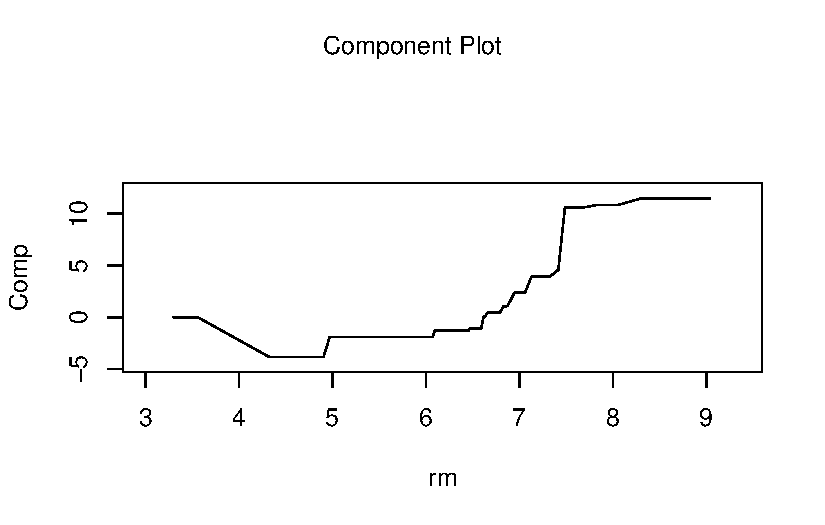
\includegraphics{aglm_files/figure-pdf/plot.aglm-1.pdf}

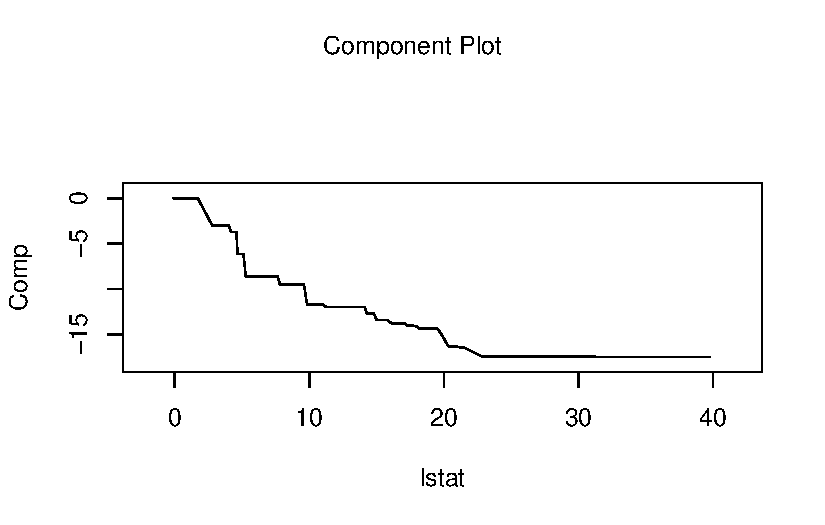
\includegraphics{aglm_files/figure-pdf/plot.aglm-2.pdf}

\section{最適な λ を探索しながら AGLM
モデルを構築する}\label{ux6700ux9069ux306a-ux3bb-ux3092ux63a2ux7d22ux3057ux306aux304cux3089-aglm-ux30e2ux30c7ux30ebux3092ux69cbux7bc9ux3059ux308b}

AGLM パッケージは、ベースになっている glmnet
パッケージの機能を数多く継承しており、たとえば cv.aglm()
関数を用いることで、λ のチューニングを自動で行うことが可能です。

\begin{Shaded}
\begin{Highlighting}[]
\NormalTok{lambda\_candidates }\OtherTok{=} \FunctionTok{seq}\NormalTok{(}\AttributeTok{from =} \DecValTok{30}\NormalTok{, }\AttributeTok{to =} \DecValTok{0}\NormalTok{, }\AttributeTok{by =} \SpecialCharTok{{-}}\FloatTok{0.2}\NormalTok{)}
\NormalTok{model\_cv.aglm }\OtherTok{\textless{}{-}} \FunctionTok{cv.aglm}\NormalTok{(}
  \AttributeTok{x =}\NormalTok{ train\_X,}
  \AttributeTok{y =}\NormalTok{ train\_y,}
  \AttributeTok{alpha =} \FloatTok{0.1}\NormalTok{, }\CommentTok{\# 正則化項のαパラメーターを指定（デフォルトは1）}
  \AttributeTok{lambda =}\NormalTok{ lambda\_candidates, }\CommentTok{\# lambda の候補を指定}
  \AttributeTok{nfolds =} \DecValTok{5} \CommentTok{\# クロスバリデーションの分割数を指定}
\NormalTok{)}
\end{Highlighting}
\end{Shaded}

\begin{Shaded}
\begin{Highlighting}[]
\NormalTok{model\_cv.aglm}\SpecialCharTok{@}\NormalTok{lambda.min }\CommentTok{\# αを変えたことで最適なλの水準も変化}
\end{Highlighting}
\end{Shaded}

\begin{verbatim}
[1] 1
\end{verbatim}

\begin{Shaded}
\begin{Highlighting}[]
\NormalTok{preds\_cv.aglm }\OtherTok{\textless{}{-}} \FunctionTok{predict}\NormalTok{(model\_cv.aglm,}
                         \AttributeTok{newx =}\NormalTok{ test\_X,}
                         \AttributeTok{s =}\NormalTok{ model\_cv.aglm}\SpecialCharTok{@}\NormalTok{lambda.min)}
\NormalTok{rmse\_ }\OtherTok{=}\NormalTok{ yardstick}\SpecialCharTok{::}\FunctionTok{rmse\_vec}\NormalTok{(test\_y, preds\_cv.aglm[, }\DecValTok{1}\NormalTok{])}
\FunctionTok{ggplot}\NormalTok{(}\AttributeTok{mapping =} \FunctionTok{aes}\NormalTok{(}\AttributeTok{x =}\NormalTok{ test\_y, }\AttributeTok{y =}\NormalTok{ preds\_cv.aglm)) }\SpecialCharTok{+}
  \FunctionTok{geom\_point}\NormalTok{() }\SpecialCharTok{+}
  \FunctionTok{labs}\NormalTok{(}\AttributeTok{title =} \FunctionTok{paste}\NormalTok{(}\StringTok{"AGLM Model: RMSE ="}\NormalTok{, }\FunctionTok{round}\NormalTok{(rmse\_, }\DecValTok{6}\NormalTok{)))}
\end{Highlighting}
\end{Shaded}

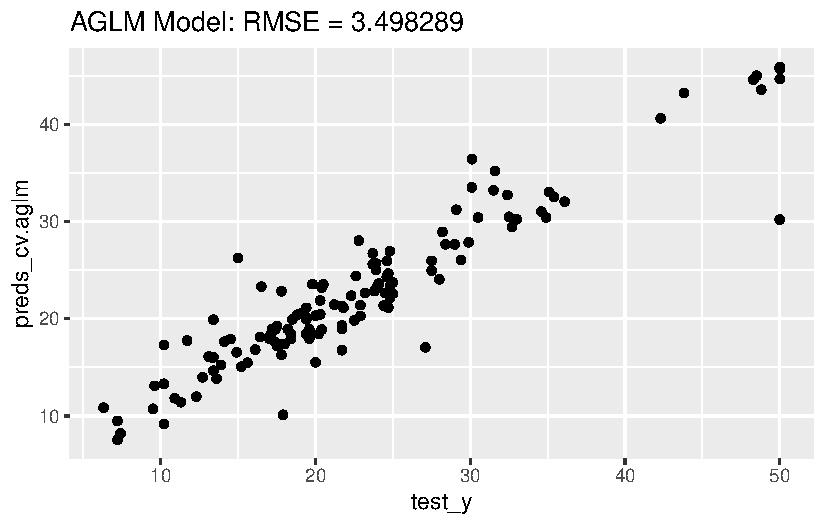
\includegraphics{aglm_files/figure-pdf/unnamed-chunk-5-1.pdf}

\section{最適な λ, α を探索しながら AGLM
モデルを構築する}\label{ux6700ux9069ux306a-ux3bb-ux3b1-ux3092ux63a2ux7d22ux3057ux306aux304cux3089-aglm-ux30e2ux30c7ux30ebux3092ux69cbux7bc9ux3059ux308b}

また、同様に cva.aglm() 関数を用いることで、λ と α
のチューニングを自動で行うこともできます。

\begin{Shaded}
\begin{Highlighting}[]
\NormalTok{lambda\_candidates }\OtherTok{=} \FunctionTok{seq}\NormalTok{(}\AttributeTok{from =} \DecValTok{30}\NormalTok{, }\AttributeTok{to =} \DecValTok{0}\NormalTok{, }\AttributeTok{by =} \SpecialCharTok{{-}}\FloatTok{0.2}\NormalTok{)}
\NormalTok{models\_cva.aglm }\OtherTok{\textless{}{-}} \FunctionTok{cva.aglm}\NormalTok{(}
  \AttributeTok{x =}\NormalTok{ train\_X,}
  \AttributeTok{y =}\NormalTok{ train\_y,}
  \AttributeTok{lambda =}\NormalTok{ lambda\_candidates, }\CommentTok{\# lambda の候補を指定}
  \AttributeTok{nfolds =} \DecValTok{5} \CommentTok{\# クロスバリデーションの分割数を指定}
\NormalTok{)}
\end{Highlighting}
\end{Shaded}

\begin{Shaded}
\begin{Highlighting}[]
\NormalTok{models\_cva.aglm}\SpecialCharTok{@}\NormalTok{alpha.min }\CommentTok{\# 最適なα}
\NormalTok{idx }\OtherTok{\textless{}{-}}\NormalTok{ models\_cva.aglm}\SpecialCharTok{@}\NormalTok{alpha.min.index }\CommentTok{\# 最適なαのインデックス番号}
\NormalTok{model\_cva.aglm }\OtherTok{\textless{}{-}}\NormalTok{ models\_cva.aglm}\SpecialCharTok{@}\NormalTok{models\_list[[idx]] }\CommentTok{\# 最適なαによるモデル}

\NormalTok{preds\_cva.aglm }\OtherTok{\textless{}{-}} \FunctionTok{predict}\NormalTok{(model\_cva.aglm,}
                          \AttributeTok{newx =}\NormalTok{ test\_X,}
                          \AttributeTok{s =}\NormalTok{ model\_cva.aglm}\SpecialCharTok{@}\NormalTok{lambda.min)}
\NormalTok{rmse\_ }\OtherTok{=}\NormalTok{ yardstick}\SpecialCharTok{::}\FunctionTok{rmse\_vec}\NormalTok{(test\_y, preds\_cva.aglm[, }\DecValTok{1}\NormalTok{])}
\FunctionTok{ggplot}\NormalTok{(}\AttributeTok{mapping =} \FunctionTok{aes}\NormalTok{(}\AttributeTok{x =}\NormalTok{ test\_y, }\AttributeTok{y =}\NormalTok{ preds\_cv.aglm)) }\SpecialCharTok{+}
  \FunctionTok{geom\_point}\NormalTok{() }\SpecialCharTok{+}
  \FunctionTok{labs}\NormalTok{(}\AttributeTok{title=}\FunctionTok{paste}\NormalTok{(}\StringTok{"AGLM Model: RMSE ="}\NormalTok{, }\FunctionTok{round}\NormalTok{(rmse\_, }\DecValTok{6}\NormalTok{)))}
\end{Highlighting}
\end{Shaded}

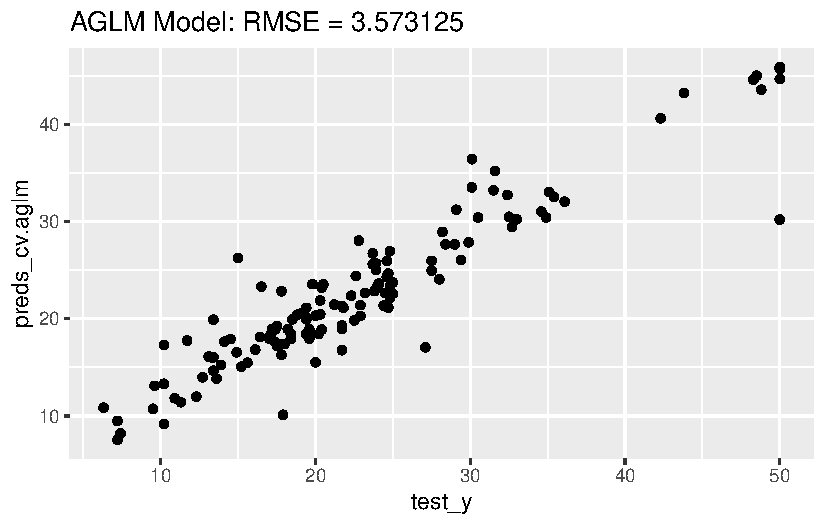
\includegraphics{aglm_files/figure-pdf/unnamed-chunk-7-1.pdf}

\bookmarksetup{startatroot}

\chapter{ALEPlot}\label{aleplot}

\section{パッケージの概要}\label{ux30d1ux30c3ux30b1ux30fcux30b8ux306eux6982ux8981-2}

ALEPlot パッケージは、予測モデルとデータをもとに、ALE (Accumulated Local
Effects、累積局所効果) を可視化する機能を実装したパッケージです。

なお、ALE は、関心のある説明変数 \(X\) について、それが取りうる値の分割
\([x_{[0]}, x_{[1]}), [x_{[1]}, x_{[2]}), ...\)
を考え、各区間について、そこに含まれるデータの \(X\)
の値を区間の両端の値に置き換えたときの予測値の増分の平均値をその区間の局所効果とみなし、区間ごとの局所効果を累積させることで、変数
\(X\) の影響を \(X\) に関する1変数関数として表現する手法です。

手法の詳細については、たとえば、「解釈可能な機械学習」に関するウェブ版書籍（Molnar著、株式会社HACARUS訳）の解説~\hyperref[0]{https://hacarus.github.io/interpretable-ml-book-ja/ale.html}
などをご参照ください。

\begin{Shaded}
\begin{Highlighting}[]
\FunctionTok{data}\NormalTok{(Boston, }\AttributeTok{package =} \StringTok{"MASS"}\NormalTok{)}
\FunctionTok{library}\NormalTok{(parsnip) }\CommentTok{\# 予測モデルの構築}
\FunctionTok{library}\NormalTok{(dplyr) }\CommentTok{\# データフレームの操作}

\CommentTok{\# ランダムシードを固定する}
\FunctionTok{set.seed}\NormalTok{(}\DecValTok{42}\NormalTok{)}

\CommentTok{\# 予測モデルを構築する}
\NormalTok{model }\OtherTok{\textless{}{-}} \FunctionTok{boost\_tree}\NormalTok{() }\SpecialCharTok{\%\textgreater{}\%}
  \FunctionTok{set\_mode}\NormalTok{(}\StringTok{\textquotesingle{}regression\textquotesingle{}}\NormalTok{) }\SpecialCharTok{\%\textgreater{}\%}
  \FunctionTok{fit}\NormalTok{(medv}\SpecialCharTok{\textasciitilde{}}\NormalTok{., }\AttributeTok{data =}\NormalTok{ Boston)}

\FunctionTok{summary}\NormalTok{(model)}
\end{Highlighting}
\end{Shaded}

\begin{verbatim}
             Length Class       Mode
lvl          0      -none-      NULL
spec         7      boost_tree  list
fit          9      xgb.Booster list
preproc      4      -none-      list
elapsed      1      -none-      list
censor_probs 0      -none-      list
\end{verbatim}

\section{ALEプロットを作成する（ALEPlot）}\label{aleux30d7ux30edux30c3ux30c8ux3092ux4f5cux6210ux3059ux308baleplot}

\texttt{ALEPlot()} 関数を使えば、ALE プロットを描画することができます。

ここで、\texttt{pred.fun} に渡す予測用の関数は、\texttt{X.model} と
\texttt{newdata}
を入力すると予測値を数値ベクトルとして出力するようなものであることが必要です。\texttt{lm}
を含む多くのモデルでは、モデルに対応する \texttt{predict}
関数のメソッドが数値ベクトルを出力するため、\texttt{pred.fun\ =\ predict}
としておけば動作します。\texttt{predict}
の返り値がベクトルでないようなクラスのモデルでは、以下のように適切に定義することが必要です。

\begin{Shaded}
\begin{Highlighting}[]
\FunctionTok{library}\NormalTok{(ALEPlot)}

\CommentTok{\# ALEPlot関数の \textasciigrave{}X\textasciigrave{} に渡す説明変数Xを用意する}
\NormalTok{X }\OtherTok{\textless{}{-}} \FunctionTok{select}\NormalTok{(Boston, }\SpecialCharTok{{-}}\NormalTok{medv)}

\CommentTok{\# ALEPlot関数の \textasciigrave{}pred.fun\textasciigrave{} に渡す予測のための関数を定義する}
\NormalTok{pred\_parsnip }\OtherTok{=} \ControlFlowTok{function}\NormalTok{(X.model, newdata)\{}
  \FunctionTok{predict}\NormalTok{(X.model, }\AttributeTok{new\_data =}\NormalTok{ newdata)}\SpecialCharTok{$}\NormalTok{.pred}
  \CommentTok{\# 予測値をベクトルとして抽出}
\NormalTok{\}}

\CommentTok{\# ALEPlotを描画する}
\NormalTok{ale }\OtherTok{\textless{}{-}} \FunctionTok{ALEPlot}\NormalTok{(X, model, pred\_parsnip, }\AttributeTok{J =} \StringTok{"rm"}\NormalTok{, }\AttributeTok{K =} \DecValTok{50}\NormalTok{)}
\end{Highlighting}
\end{Shaded}

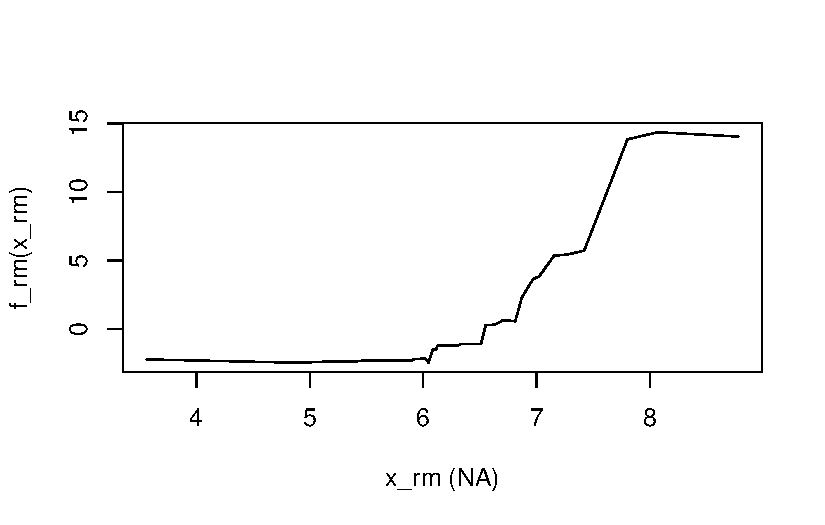
\includegraphics{ALEPlot_files/figure-pdf/ALEPlot-1.pdf}

DALEXパッケージがインストール済みの場合は、DALEX::yhat()
関数を利用することもできます。この関数は、ALEPlot()
関数が要求するのと同じ引数名で定義されており、しかも、かなり広範な種類の予測モデルに対応しています。

\begin{Shaded}
\begin{Highlighting}[]
\CommentTok{\# 2次元ALEPlotを描画する}
\NormalTok{ale}\FloatTok{.2}\NormalTok{d }\OtherTok{\textless{}{-}} \FunctionTok{ALEPlot}\NormalTok{(X, model, DALEX}\SpecialCharTok{::}\NormalTok{yhat, }\FunctionTok{c}\NormalTok{(}\StringTok{"rm"}\NormalTok{, }\StringTok{"dis"}\NormalTok{))}
\end{Highlighting}
\end{Shaded}

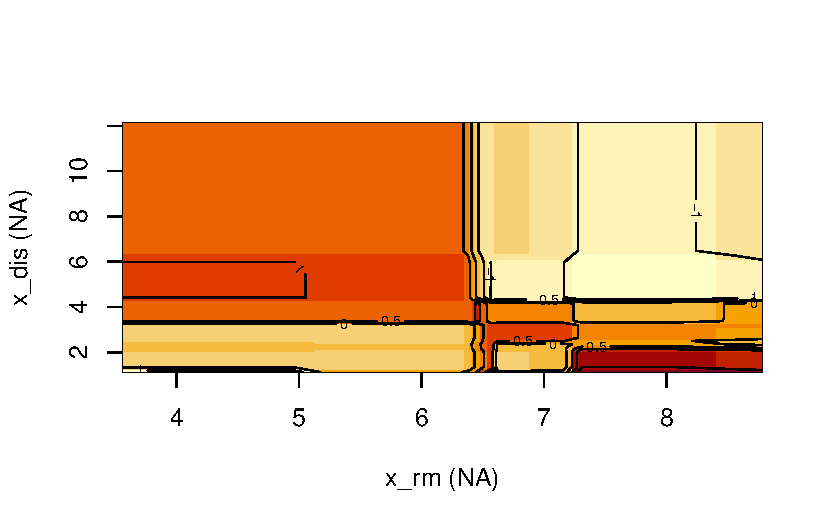
\includegraphics{ALEPlot_files/figure-pdf/unnamed-chunk-2-1.pdf}

標準のプロットは R
のグラフィックス関数で作成されますが、返り値をデータフレーム化することで、ggplot2
パッケージで ALE を可視化することもできます。

\begin{Shaded}
\begin{Highlighting}[]
\FunctionTok{library}\NormalTok{(ggplot2)}

\FunctionTok{ggplot}\NormalTok{(}\AttributeTok{data =} \FunctionTok{as.data.frame}\NormalTok{(ale[}\DecValTok{2}\SpecialCharTok{:}\DecValTok{3}\NormalTok{]),}
       \FunctionTok{aes}\NormalTok{(}\AttributeTok{x =}\NormalTok{ x.values, }\AttributeTok{y =}\NormalTok{ f.values)) }\SpecialCharTok{+}
  \FunctionTok{geom\_line}\NormalTok{() }\SpecialCharTok{+} \FunctionTok{geom\_point}\NormalTok{()}
\end{Highlighting}
\end{Shaded}

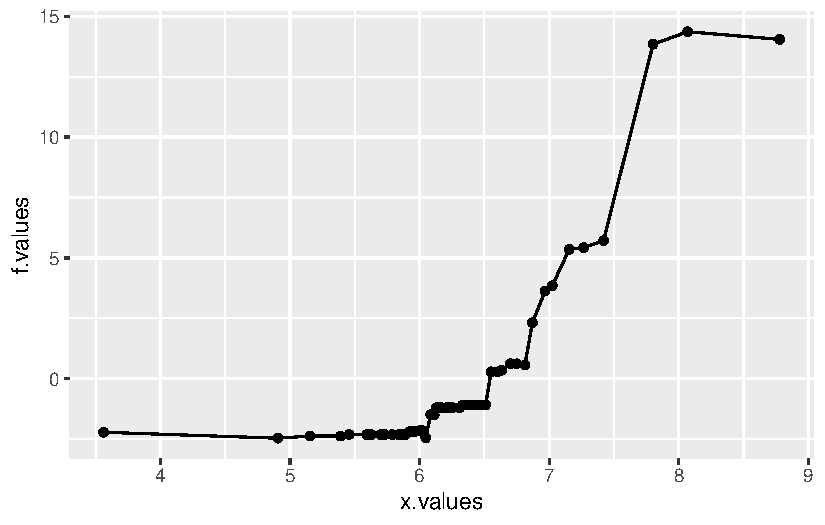
\includegraphics{ALEPlot_files/figure-pdf/aleplot_gg-1.pdf}

\section{PDプロットを作成する（PDPlot）}\label{pdux30d7ux30edux30c3ux30c8ux3092ux4f5cux6210ux3059ux308bpdplot}

PD プロットを作成するための関数 \texttt{PDPlot()} を用いれば、PD
を描画することもできます。基本的な使い方は \texttt{ALEPlot()}
関数と同じです。

なお、PD は、ALE
と同様に、予測モデルにおける特定の特徴量の効果を解釈するための手法です。詳細については、前掲のウェブ書籍の解説
\url{https://hacarus.github.io/interpretable-ml-book-ja/pdp.html}~などをご参照ください。

\begin{Shaded}
\begin{Highlighting}[]
\CommentTok{\# PDPlotを描画する}
\NormalTok{pdp }\OtherTok{\textless{}{-}} \FunctionTok{PDPlot}\NormalTok{(X, model, pred\_parsnip, }\StringTok{"rm"}\NormalTok{, }\DecValTok{20}\NormalTok{)}
\end{Highlighting}
\end{Shaded}

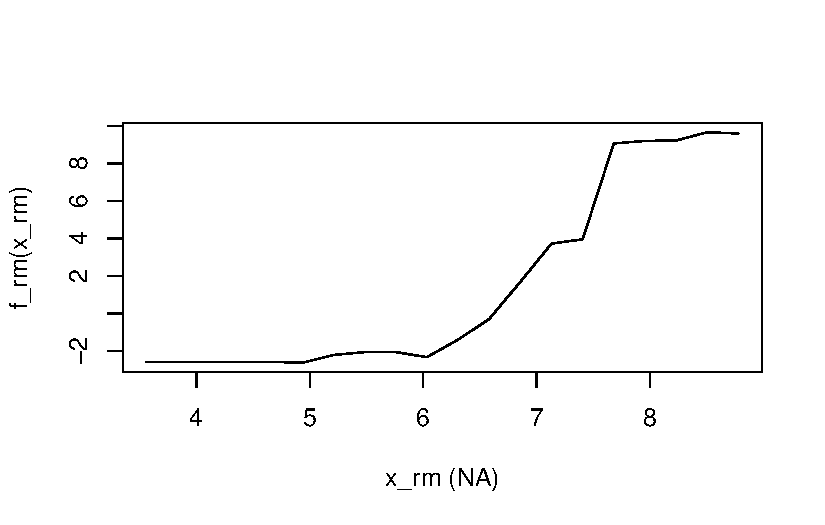
\includegraphics{ALEPlot_files/figure-pdf/PDPlot-1.pdf}




\end{document}
